\chapter{Implementation Details ESP32}
In this chapter are reported all steps that have been done in order to understand the functionality of ESP-IDF provided by Espressif\cite{ESP-IDF-Page} in order to achieve the goal of the assignment and create the final project presented at the end of the course.
After a general brainstorming, an ESP32 was decided as the chosen board because many useful resources are freely available. Mainly ESP-IDF that is Espressif’s official IoT Development Framework for the ESP32, ESP32-S and ESP32-C series of SoCs. It provides a self-sufficient SDK for any generic 
application development on these platforms, using programming languages such as C and C++.

\section{WireGuard on ESP32}\label{sec:wireguard}

In order to make the ESP32 board able to connect through a VPN tunnel, it is necessary to set up a WireGuard module. This module, as described before, is used to interface the board with the remote server, so related IPs needs to be consistent with the one in the server.\\ 
The WireGuard module \texttt{trombik\_esp\_wireguard} was taken from the Trombik project \cite{wg_trombik} and added in the directory \texttt{Esp32\_tcpprompt\_wg/components}.\\
Then the following line:
\begin{lstlisting}
{REQUIRES trombik\_esp\_wireguard nvs\_flash}   
\end{lstlisting}
was inserted in the file \texttt{CMakeLists.txt} in the directory \texttt{Esp32\_tcpprompt\_wg/main}.\\




\subsection{Related projects}
First of all, it is better to introduce the main projects that was the starting point reference:
\begin{itemize}
    \item Smartalock \cite{wg_smartalock}, which is a C WireGuard implementation for lwIP, which cointains a generic structure (i.e. independent from the platform). 
    As explained in its Readme document the code has four main portions:
    \begin{itemize}
        \item \texttt{wireguard}, which contains the bulk of the WireGuard protocol code and is not specific to any particular IP stack
        \item \texttt{wireguardif}, which contains the lwIP integration code and makes a netif network interface and handles periodic tasks such as keepalive/expiration timers
        \item \texttt{wireguard-platform}, which contains the definition of four functions to be implemented per platform 
        \item \texttt{crypto}, which supports:
        \begin{itemize}
            \item BLAKE2S
            \item X25519
            \item CHACHA20-POLY1305  
        \end{itemize}   
    \end{itemize}
More details on the cryptographic algorithms are discussed in the background chapter (\ref{sec:WGAlgo}).
    \item Trombik \cite{wg_trombik}, is an alpha extension of the previous project, and creates a single WireGuard peer connection using ESP-IDF. This module is also a component of the project that has all the necessary to adapt the Smartalock to an ESP32 board. 
\end{itemize}



\subsection{WireGuard module}
In order to set up the module, the starting point was the ping example present in the Trombik project \cite{wg_trombik}, in order to see if the WireGuard server was reachable. To do that, has been tried the provided example configured with all the parameters like the one on the server.
This example could be divided in:
\begin{itemize}
    \item WireGuard configuration and setup, where all the WireGuard parameters are initialized in \texttt{wireguard\_setup()}, setting:
    \begin{itemize}
        \item private\_key
        \item listen\_port
        \item public\_key
        \item allowed\_ip
        \item allowed\_ip\_mask
        \item endpoint      
        \item port
        \item persistent\_keepalive (i.e. periodically send keepalive packets)
    \end{itemize}
    and then are called:
    \begin{itemize}
        \item \texttt{esp\_wireguard\_init()}, which received the previous variables
        \item \texttt{esp\_wireguard\_connect()}, connects to the corresponding peer 
    \end{itemize}
    \item WiFi and ping, that connects the module to the WiFi and manages the ping communication with server. The WiFi is connected using \texttt{wifi\_init\_sta()} that calls one of the two following functions:
    \begin{itemize}
        \item \texttt{wifi\_init\_tcpip\_adaptor()}
        \item \texttt{wifi\_init\_netif()} 
    \end{itemize}
    the ping instead is managed by \texttt{start\_ping()}, which communicates with the server and respond with a timeout or a success.
    \item time synchronization, necessary to agree during the communication with the server (it is managed by the sync\_time.c)
    \item main, which manages the previous sections in order to run the example and ping the server.
\end{itemize}   
Starting from this configuration, the example provided is used as a reference to build the application.

\subsection{Failed approach}
In a first attempt it was tested also another project from Zmeiresearch \cite{wg_zmeiresearch}, but it was unfeasible to make it work. In a comparison with Trombik it was noticed that maybe it could be due to the absence of a timing synchronization. 

\section{Blinky, Wifi, Component logic}
The first step was to make something run on the ESP32 to understand how the system works. Read the Espressif Documentation for ESP-IDF and for the ESP32 was essential.
Following the guide provided in the Appendix \ref{sec:SysSetupESP32} , a Blinky project was tested. Its directory location is provided here:
\begin{lstlisting}
    esp-idf/examples/get-started/hello_world
\end{lstlisting} 

By doing this the good state of the board was checked.
The next step was to establish an internet connection between the ESP32 and another machine in order to add later the VPN tunnel.
In order to do that a TCP/IP connection was chosen and so implemented starting from the \texttt{Hello\_World} project.
But before that, the WiFi connection needed to be done. The ESP-IDF provides a project where this functionality is provided.
\begin{lstlisting}
    esp-idf/examples/common_components/protocol_examples_common
\end{lstlisting}

In a first attempt the \textit{protocol\_examples\_common} project was included as a component inside the \textit{TCP/IP} project (to understand how to add a component into a project look at the official documentation \cite{ESPcomponents})
\\Then the WireGuard module was analysed starting from two projects described in section \ref{sec:wireguard} in more details. Those two projects were tested standalone and at the end
the Trombik\cite{wg_trombik} project was added as a component in the TCP/IP project. As written in the next section \ref{sec:VPNproject}, in the final version of the project called \texttt{Esp32\_tcpprompt\_wg} the WiFi functions already integrated inside Trombik project were used instead of the WiFi component provided by Espressif. 

\section{TCP/IP communication with WireGuard on ESP32}\label{sec:VPNproject}
After the previous examples, that were propaedeutic to the development of the project, it was possible to implement a TCP/IP communication inside a VPN tunnel.\\ 
The project is located in the directory \texttt{/Esp32\_tcpprompt\_wg}.\\
The task developed for the communication is the following one, and it is located in the file \texttt{main.c}, inside the directory 
\texttt{/Esp32\_tcpprompt\_wg/main}:
\begin{itemize}
    \item \texttt{static void tcp\_client\_task(void *pvParameters)}\\ It contains the main loop of the application, in which there can be found the four main functions:
     \begin{enumerate}
        \item \texttt{socket()} : it creates a TCP socket
        \item \texttt{connect()} : it opens the TCP connection
        \item \texttt{send()} : it sends a message
        \item \texttt{recv()} : it receives a message 
    \end{enumerate}
    In this task it is set which port needs to be used in listening. The one used in this project is 3333.\\
    When the TCP socket is opened, the communication starts and makes possible to have an interaction between the esp32 and the server.\\
    The application that was created was a login-like communication, so the ESP32 asks for some credentials and the user answers.\\
    The ESP32 has a static list of available commands:
    \begin{itemize}
        \item \texttt{Hello from ESP32, please login Username:}\\
        It is the first message sent by the ESP32 which waits for an answers with the user credential. 
        \item \texttt{Password:}\\
        After receiving the username it asks for a password, and waits for the user to answer.
        \item \texttt{Authentication succeeded\\
         Select commands:\\
        - Hello:  to get greetings\\
        - Usage:  to read cpu load\\
        - LogOut: Log Out}\\
        If the combination of username and password are correct, the user can choose one of these commands and will have a different answer.\\
        \item \texttt{Authentication failed, try again...  Username: }\\
        If the username or the password (or both) is wrong, the authentication failed and the esp32 asks again for the credentials.
    \end{itemize}
    
\end{itemize}
After developing this task, the WiFi module and the WireGuard module were taken from Trombik\cite{wg_trombik} and added to our project.\\
When the project is run, the function \texttt{main()} is called and it calls the functions:
\begin{enumerate}
    \item \texttt{wifi\_init\_sta()} : it initializes the WiFi module
    \item \texttt{wireguard\_setup()} : it setups the WireGuard server
    \item \texttt{xTaskCreate()} : it is a FreeRTOS function that receive a task that needs to be created. In this case it receives the \texttt{tcp\_client\_task}
\end{enumerate}
It also checks the time for the timing synchronization, that is necessary for the handshake.
\\An example of the communication can be seen in figure \ref{fig:communicationEx}.
    
\begin{figure}[H]
    \centering
    \vspace{0.35cm}
    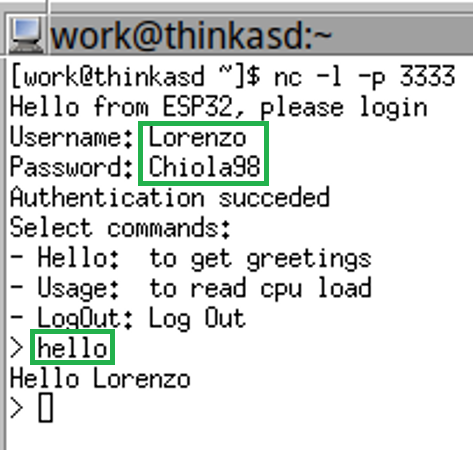
\includegraphics[width=0.4\textwidth]{images/communicationEx.png}
    \caption{Communication output}
    \label{fig:communicationEx} % This is the image label, with which you can refer to the image in any document location.
\end{figure}

It could be seen that the messages sent by the esp32 are the one listed before, and for each of them there is the user answer (the message in the green box).\\


\section{Adding the WireGuard module to iperf and testing performance}\label{sec:iperf_wg}

Between the code examples of ESP-IDF there is an iperf port for the ESP32, available at

\texttt{examples/wifi/iperf/}\\(the actual iperf code is inside a submodule located at \texttt{examples/common\_components/iperf/}).\\
iperf is a common tool used to measure network throughput between two hosts. One will run the tool in server mode, the other in client mode. Random packets of data will be exchanged by the two instances (over TCP by default) to measure the average speed.\\
The iperf port by Espressif is based on another one of their code examples: a command line interface provided over the serial port. Its code is available at

\texttt{examples/system/console/advanced/components/}, which is included as a submodule in iperf. The available commands are iperf itself, \texttt{sta} and \texttt{ap} to configure the WiFi connection (station or access point), and \texttt{free} and \texttt{heap} to measure free ram (in the present or the historical low). A new command can be registered to the console, together with a callback which works much like \texttt{main(int argc, char* argv[])} with arguments passed from the command line.\\
The following procedure shows how to add the WireGuard module from the repository \cite{wg_trombik} to iperf for the ESP32, also adding a command to the text interface.\\
The result should be similar to the contents of the folder \texttt{iperf\_wg/} of the supplied code. It can be useful to compare this folder to the iperf code from ESP-IDF to highlight the differences introduced with the WireGuard module.\\
It is assumed that the provided iperf example was built as a standard ESP32 project without issues.

\begin{enumerate}
    \item Mkdir \texttt{components/} and git clone \cite{wg_trombik} in that folder. The \texttt{components/} folder, if it exists, is automatically searched for submodules by the build system. The only constraint is that a valid \texttt{components/*/CMakeLists.txt} file has to be present for each submodule.
    \item Move the time synchronization code
    
    \texttt{components/esp\_wireguard/examples/demo/main/sync\_time.c / .h} to \texttt{main/}. The rest of the \texttt{examples/demo/} folder can be deleted.
    \item Register a new command to set up the VPN. Take \texttt{main/cmd\_wifi.c / .h} as an example to adhere to the structure of the underlying iperf code. Files \texttt{main/cmd\_wifi.c / .h} were written this way. The new command \texttt{wgup [peer ip address]} starts the VPN tunnel to the other peer. The call-back function is \texttt{wg\_up()}, while the function \texttt{register\_wg()} registers the new command in the command line at start-up.
    \item Integrate the new code in the project:
    \begin{itemize}
        \item As always when adding new source files, it is necessary to add them to the
        
        \texttt{main/CMakeLists.txt} project file so they can be compiled. Add each file name in double quotes after the last C source in the \texttt{idf\_component\_register(SRC "...")} macro.
        \item Include the new header file inside the aggregator header \texttt{cmd\_decl.h}.
        \item Call \texttt{register\_wg()} inside \texttt{app\_main()} to register the new command.
    \end{itemize}
    \item Optionally use the \texttt{menuconfig} system to define options for the WireGuard module. In the supplied code this system is used, so an additional file \texttt{main/Kconfig.projbuild} was created to define some new menu entries which will appear inside the configuration along with the standard options.
\end{enumerate}

It will be now possible to use the command line interface through the serial port monitor.\\
Iperf will work as before, but it will be possible to send the \texttt{wgup} command to set up the VPN tunnel, so that any further traffic originating from the inside of the esp32 will be routed through the tunnel.\\
\ref{fig:iperf_wg_long} is a screenshot of the serial monitor session after running iperf, starting the VPN, and running iperf again this time inside the VPN tunnel. Note that the IP address changes for the second run; also the IP address of the first iperf server is the same as the IP address of the WireGuard peer, since they were running on the same computer.
This run was used to record performance and RAM usage, see \ref{sec:performance}.

\begin{figure}[H]
    \centering
    \vspace{0.5cm}
    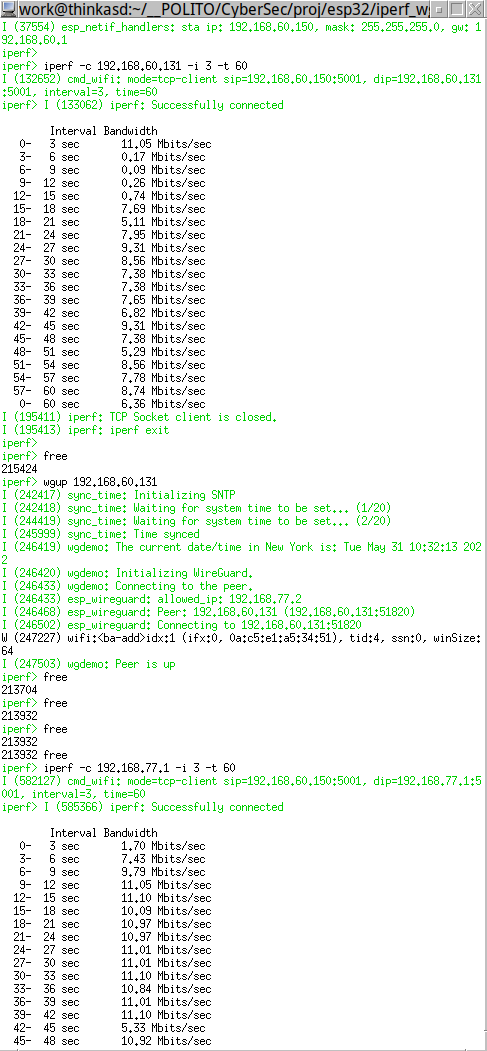
\includegraphics[ width=0.4\textwidth]{images/iperf_wg_serial_monitor_long.png}
    \caption{iperf running on the ESP32 both outside and inside the VPN tunnel. The remote computer is reachable both from inside and outside the VPN, it is running iperf in server mode: \texttt{iperf -s}}
    \label{fig:iperf_wg_long} % This is the image label, with which you can refer to the image in any document location.
\end{figure}


